\chapter{Parameter Lock Record  Page:}
The RLCK Page is used to record Parameter Locks in real-time. If the sequencer is running, any parameter changes on the MD will be recorded.\\
\\
\fbox{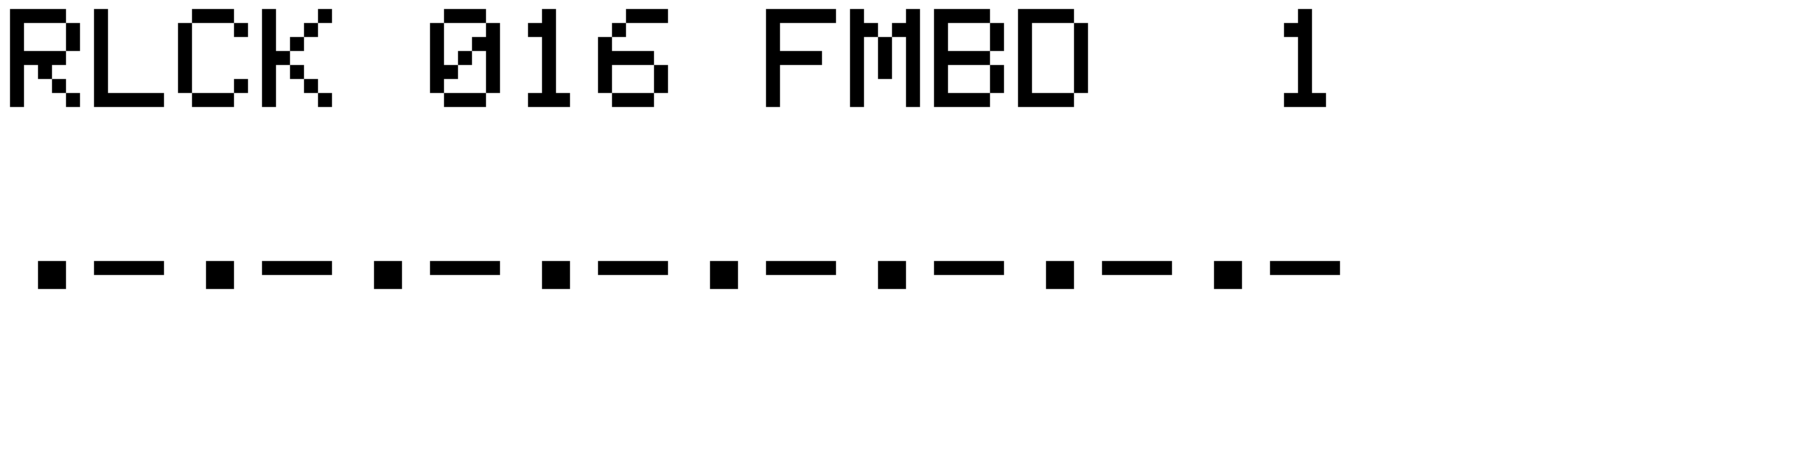
\includegraphics[scale=.40]{rlck_page_init.png}}\\
\textit{To enter the RLCK Page: Enter the RTRK Edit mode by pressing \textbf{[ Encoder 2 ]} from the Grid Page. Press the \textbf{[ Save ]} button to enter RLCK mode.}
\section{Parameter MIDI Learn}
Any MD parameter changes in the RLCK Page will be automatically learned. If a free parameter lock slot is available, it will automatically be assigned to the last Parameter received. \\
\\
When in RLCK Page, the current sequencer Track will automatically change according to the track of the last MD Parameter modified. 

\section{Encoder Assignment:}
\begin{itemize}
	\item \textbf{[ Encoder 1 ]: } --
	\item \textbf{[ Encoder 2 ]: } --
	\item \textbf{[ Encoder 3 ]: } Track Length
	\item \textbf{[ Encoder 4 ]: } --
\end{itemize}
\section{Clearing:}
\begin{itemize}
\item To clear the current track of all parameter locks, press the \textbf{[ Write ] }(top right)
\item \\To clear all MD tracks of all parameter locks,  press \textbf{[ Shift2 ] + [ Write ]}
\end{itemize}
\section{Rotating visible sequence:}
Each track consists of 4 pages of 16 steps, for a total of 64 steps per track.
\begin{enumerate}
	\item Rotate the current track-page by pressing the \textbf{[Shift1] }button.
\end{enumerate}
\section{Changing track length:}
\begin{enumerate}
	\item Track length is controlled by rotating \textbf{[ Encoder 3 ]}. Only steps less than the current track length are drawn.
	\item To change the lengths of all 16 tracks simultaneously hold down \textbf{[Shift 2]} whilst rotating \textbf{[ Encoder 3 ]}.
\end{enumerate}
